\chapter{Results interpretation}

Based on the results of the different experiments I made, I will try to answer in this chapter to three main questions:
\begin{enumerate}
  \item Compared to other available solutions, how good is the current configuration chosen by INGInious to face the responsiveness challenge of the platform?  How much better could it be?  How easy would it be to improve it?
  \item Could there be a solution tailor-made for the specific case of INGInious?  What would it be?  What would it take to use it?
  \item What would be the cost of providing a stronger/safer isolation to the containers used by INGInious?  What opportunities could it bring?
\end{enumerate}

\section{Current INGInious situation}
We will here consider the first question:
\begin{center}
  \say{\textit{Compared to other available solutions, how good is the current configuration chosen by INGInious to face the responsiveness challenge of the platform?  How much better could it be?  How easy would it be to improve it?}}
\end{center}

The current configuration of INGInious is the following:
\begin{center}
\begin{tabular}{rl}
  \textbf{Container manager} & Docker \\
  \textbf{Base image} & Centos \\
  \textbf{Storage driver} & overlay2 \\
  \textbf{Container runtime} & runc \\
  \textbf{Control group version} & v1 \\
  \textbf{Rootless containers} & no \\
\end{tabular}
\end{center}

This configuration is quite decent, and gives good performances, their is mainly one change that can improve those.  But let's analyse this step by step.

\subsubsection{Storage driver}
Overlay2 (referenced later as simply overlay) is the storage driver that Docker recommands to use by default (when OverlayFS is supported on the host).  Its layer mechanism allows to limit the redundancy of information when you use the same base image to create different images.  And its file-based copy-on-write strategy gives overal good performances.

\begin{figure}[h!]
  \begin{center}
    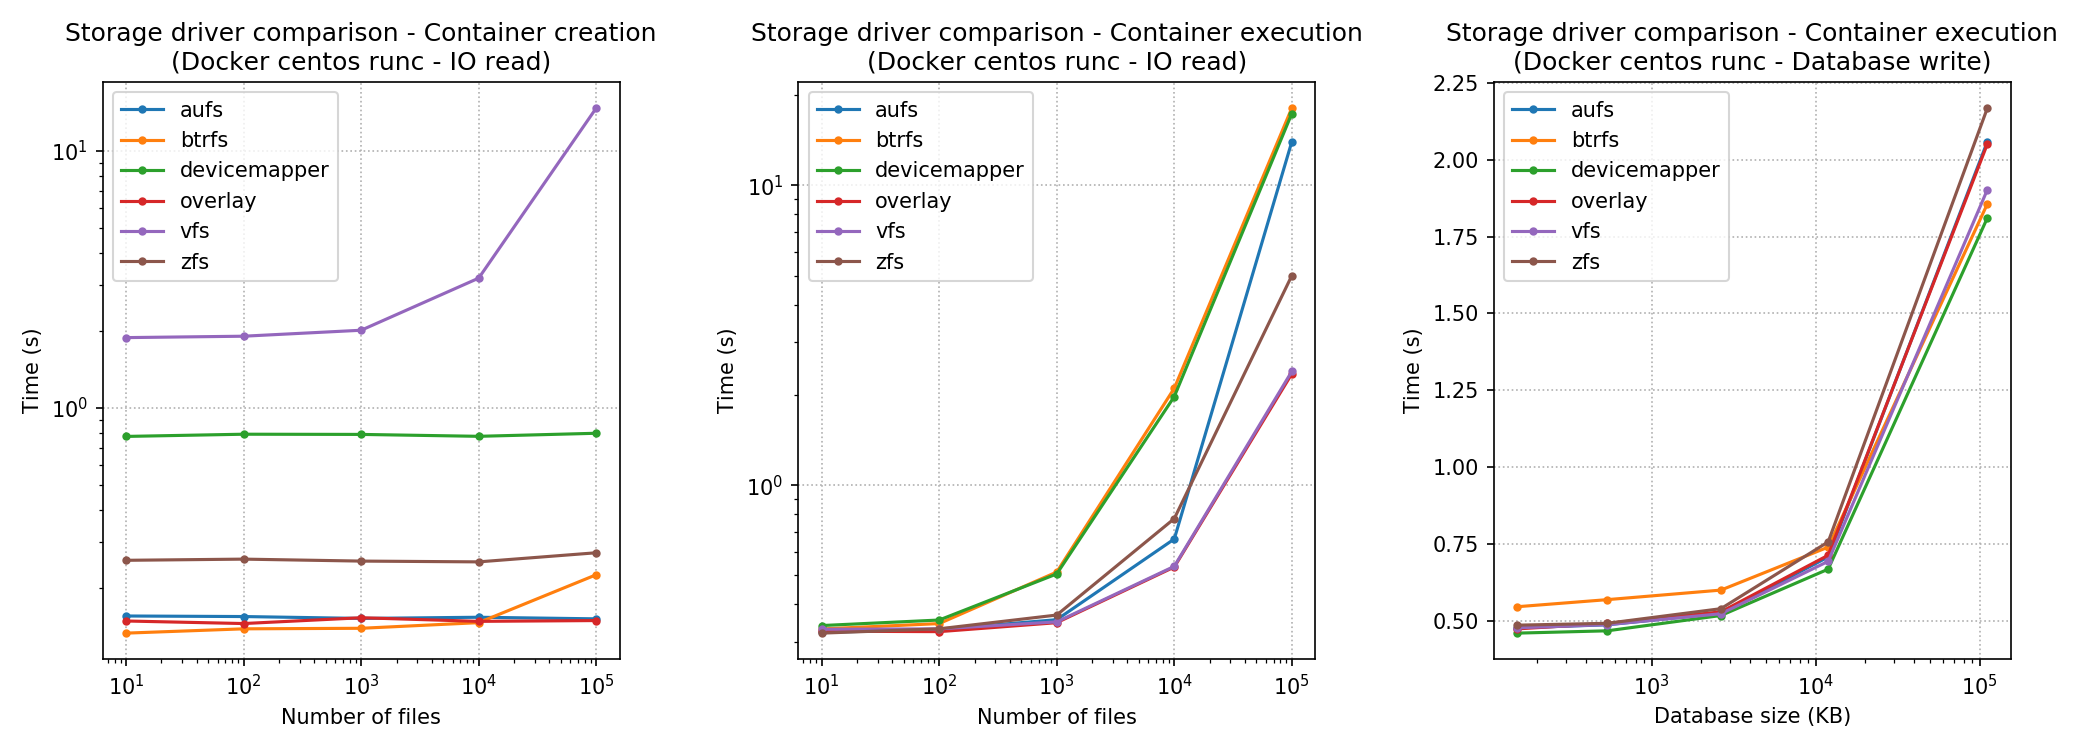
\includegraphics[width=\linewidth]{images/question-1-storage-driver.png}
    \caption{Storage driver performance comparison for Centos containers, launched with Docker and runc}
    \label{fig:q1:storage-driver}
  \end{center}
\end{figure}

On Figure \ref{fig:q1:storage-driver}, we can see how much it cost to have a full-copy mechanism like vfs for each container creation.  We can also see that overlay, aufs and btrfs offers similar performances for the creation of containers.  The main differences between those three is shown by their performance when solicitating I/O.  
\begin{itemize}
  \item Aufs, even though performing similarly to overlay in all the other cases (not shown here) and relying on the same union file system mechanism as overlay, gets far behind the latest when a lot of read operations are done.  This most likely comes from one big difference in the implementation of those two union file system: when a file is opened with OverlayFS, all the operations on it are directly managed by the underlying file systems.  This simplify the implementation, and improve the performances quite a lot as we can see on the second graph of the figure.  (For this test, for each \texttt{openat} system call, four \texttt{read} system call are done)
  \item On the last graph of the figure (on the right), we can see the advantage of using block-based copy-on-write, when modifying big files.  Indeed, when doing so, where overlay and aufs will need to copy the whole file before modifying it, the other solutions will only need to copy the file system blocks needing to be modified (or not even copy the file in the case of vfs).  We can see that devicemapper handles this a little bit better than btrfs, but given the much higher container creation cost of the first one, it will most likely be more intersting to use btrfs in most cases.
  \item One more thing to pay attention to, is that is seems that storage drivers with block-based copy-on-write mechanism, face some difficutlies when creating container with a large amount of files in it.  This might be harder to see here for devicemapper and zfs, but it is the case.  Zfs seems to also suffer from big files in the container filesystem, for the container creation.
\end{itemize}
One more reason to justify the use of overlay is that in most container use cases, read operations are the most important ones.  Normally, no large amount of data should be written in the container file systems, volumes (external storage from the host, mounted into the container file system) should specifically be used for that purpose as it provide nearly native writing performances and the data persists, even after the end of the container life cycle.

\subsubsection{Base image}

Alpine is quite popular in containers file systems.  Thanks to its minimalist default configuration, its image is really light compare to the ones of more complete file systems.  The Alpine base image provided by Docker is only $5.61$\texttt{MB}, while Centos's one is $203$\texttt{MB}.  But the size taken by images on disk isn't really something we worry about in our case.

\begin{figure}[h!]
  \begin{center}
    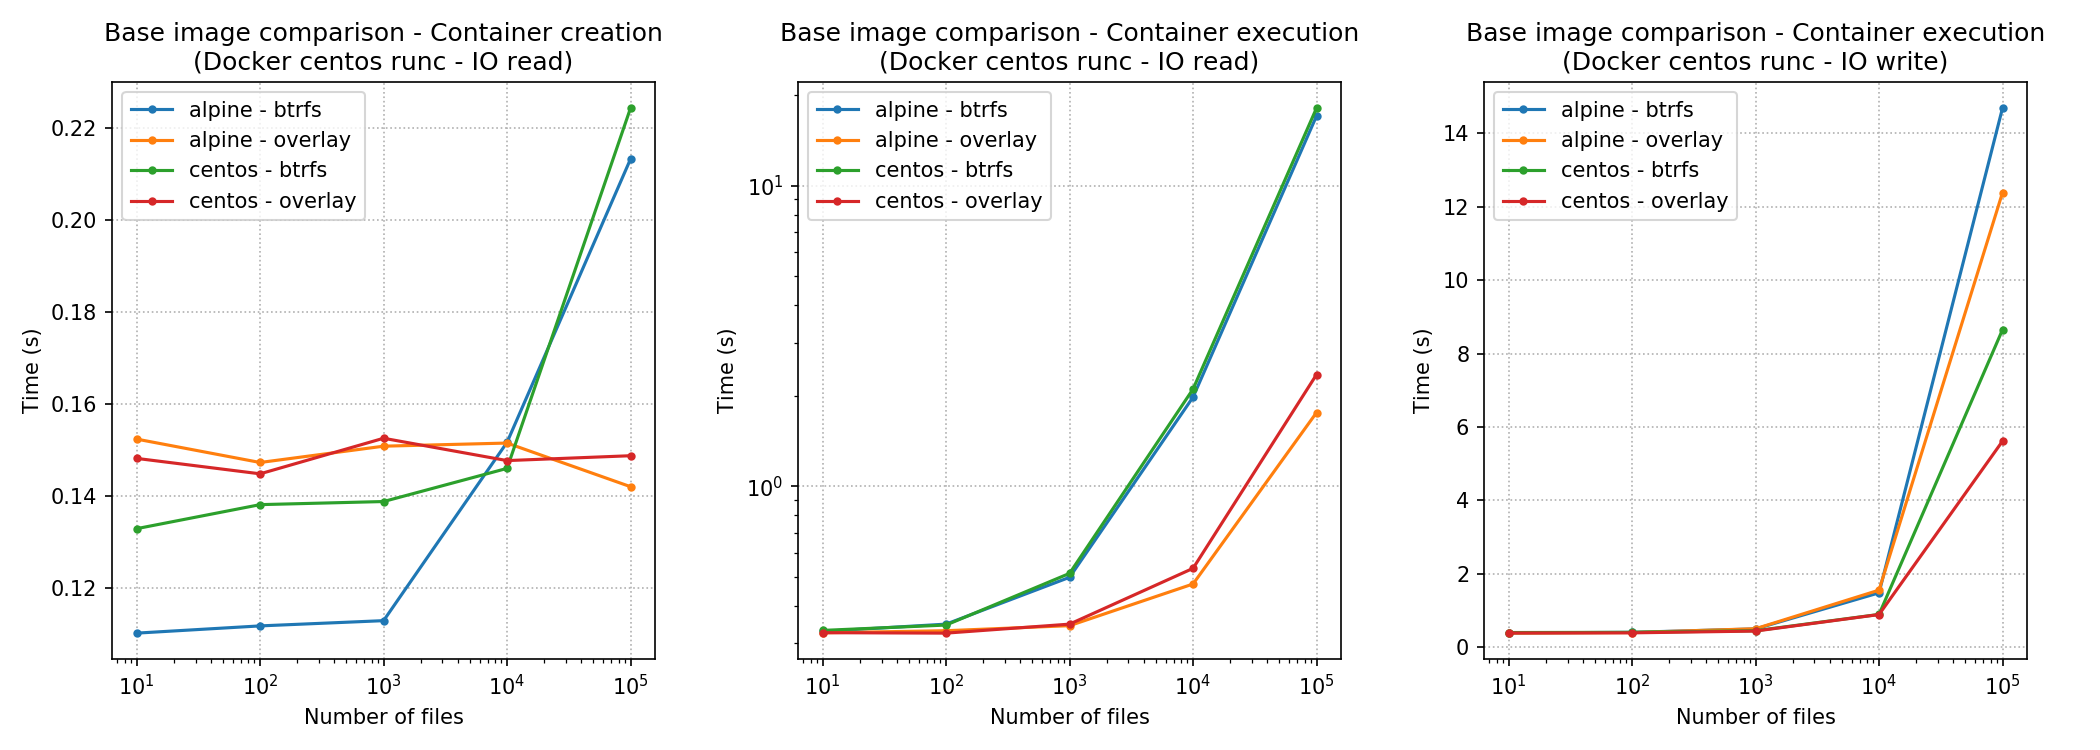
\includegraphics[width=\linewidth]{images/question-1-base-image.png}
    \caption{Base image performance comparison for containers launched with Docker and runc}
    \label{fig:q1:base-image}
  \end{center}
\end{figure}

From the graphs of Figure \ref{fig:q1:base-image}, we can notice several things:
\begin{itemize}
  \item We can see on the first graph (on the left) that, once more, btrfs offers better creation performances when the number of files is smaller.  Therefore, being a more complete linux distribution, with more functionnalities, and so, more files, Centos-based images are more costly for container creation.
  \item On the second graph, it also appears that simple read operations are a little bit faster when using Alpine as base image.  This trend has also been observed with bigger file read, with the \textit{Database read} test.
  \item One thing really interesting that we can see on last graph however, is that the trend seems to be inverted for write operations.  This difference is really likely to be caused by the difference in the implementation of \texttt{tar} (used for this test) in each distribution's package repository.  Indeed, the implementation coming from Alpine makes a lot more system calls (about three times more) than Centos's one.
\end{itemize}

The choice of Centos as base image can then be justified by the maturity of such distribution.  It had been around for a while, it is widely used outside of container applications, and is more likely to count optimization in the different tools at disposal.  If we don't require those tooles though, the minimalist and ligthweight aspect of Alpine makes it a better choice.

\subsubsection{Container runtime}

On Figure \ref{fig:q1:runtime} is chown the influence of different container runtime solutions on the different execution step of the container.  

\begin{figure}[h!]
  \begin{center}
    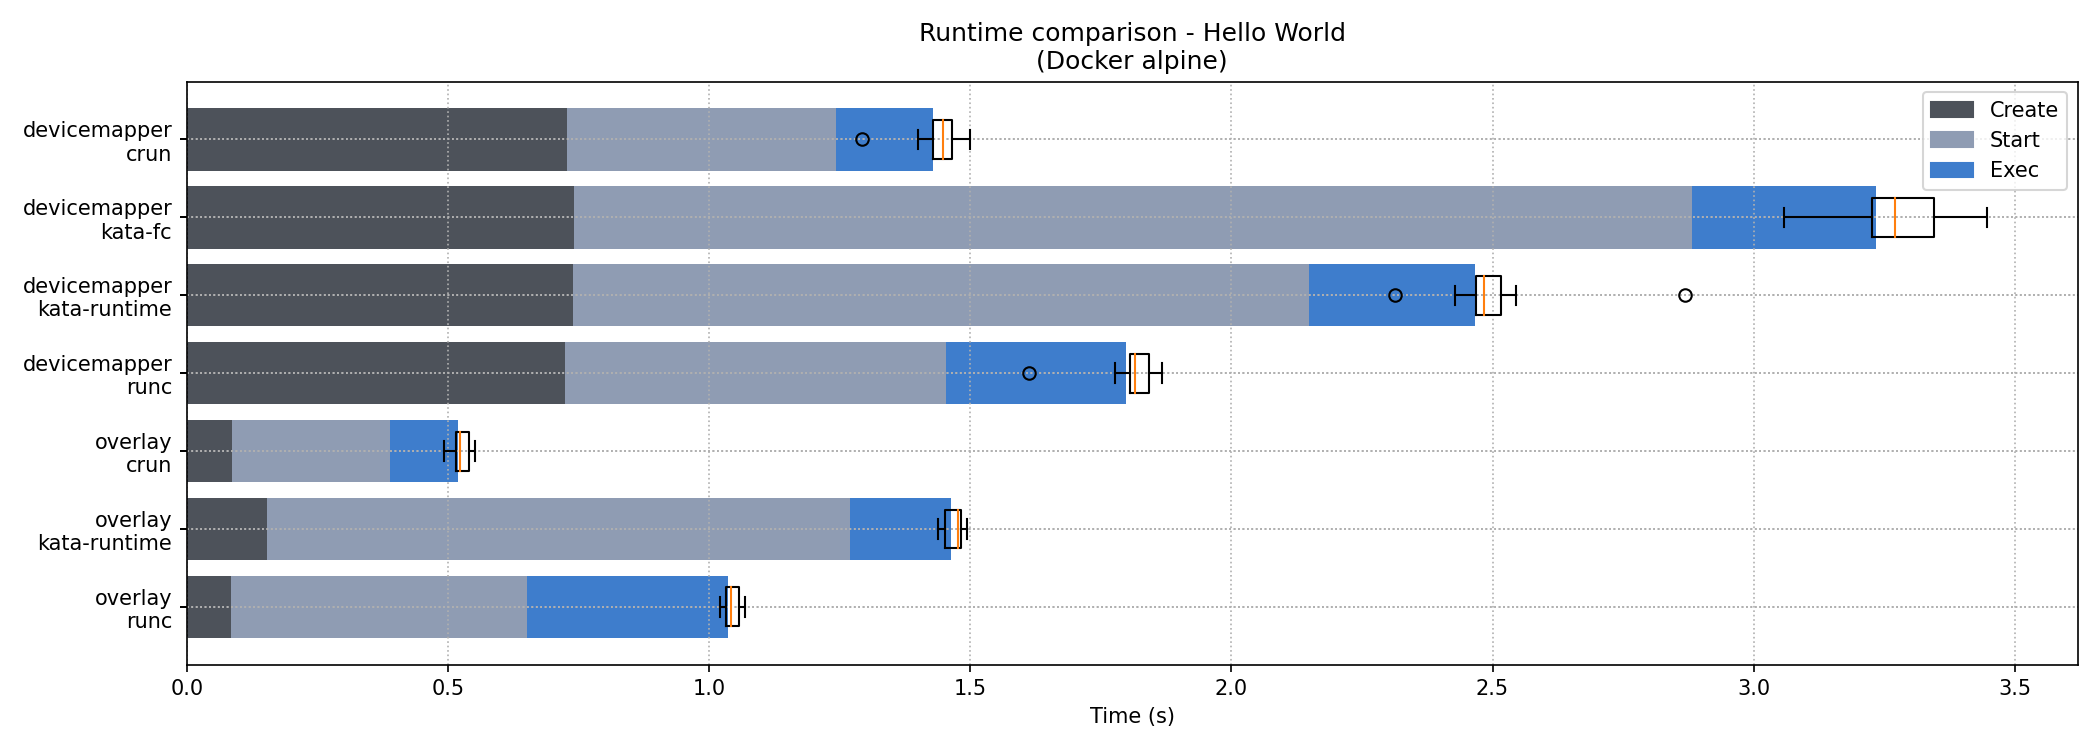
\includegraphics[width=\linewidth]{images/question-1-runtime.png}
    \caption{Runtime performance comparison for Alpine containers, launched with Docker}
    \label{fig:q1:runtime}
  \end{center}
\end{figure}

By first comparing crun to runc, we see how much of a difference it makes to use an efficient C implementation, over a less efficient Go one.  The difference is much more obvious for the \texttt{start} and \texttt{exec} phases as those are the steps where real low-level operations are made by the container runtime (entering namespaces, setting cgroups, forking processes).  

Then we have the Kata Containers solutions, based on virtualization.  It obviously will lead to a greater overhead for creating and starting containers, as a whole kernel as to be loaded.  However, the \texttt{exec} phase seem to have a much lower overhead.  We can't miss how much worse is \texttt{kata-fc} (using Firecracker hyperviser) compared to \texttt{kata-runtime}, and it might be disapointing given the recent popularity that has embrassed Firecracker.  In response to that here are some important elements:
\begin{enumerate}
  \item Firecracker has not been conceived to run under Kata Containers's hood.  It is really possible that it would perform better when running standalone.
  \item Some advantages that Firecracker has and that are not obvious in our study case are, first, the memory footprint, which is way smaller than with Qemu, and second, the reduced code base, which ensure a much lower attack surface.  Those are also reason why Firecracker is so popular.
  \item After some discussion with Kata Containers community\footnote{The full discussion can be found at this link: \href{https://github.com/kata-containers/runtime/issues/2642}{https://github.com/kata-containers/runtime/issues/2642}}, it turned out that Kata Containers make use of one feature of Qemu that Firecracker doesn't have, that would justify this difference in performance: vNVDIMM.  Thanks to vNVDIMM, the root file system of the guest VM is fully loaded in memory and directly accessed in it, which is faster than reading it from disk as Firecracker does.
\end{enumerate}

\subsubsection{Container manager}

On Figure \ref{fig:q1:manager} are shown the different container manager considered in the experiements, in their most performant configuration.  Docker and Podman using crun as runtime, and overlay or btrfs as storage driver.  LXD uses lxc as runtime and btrfs as storage driver.

\begin{figure}[h!]
  \begin{center}
    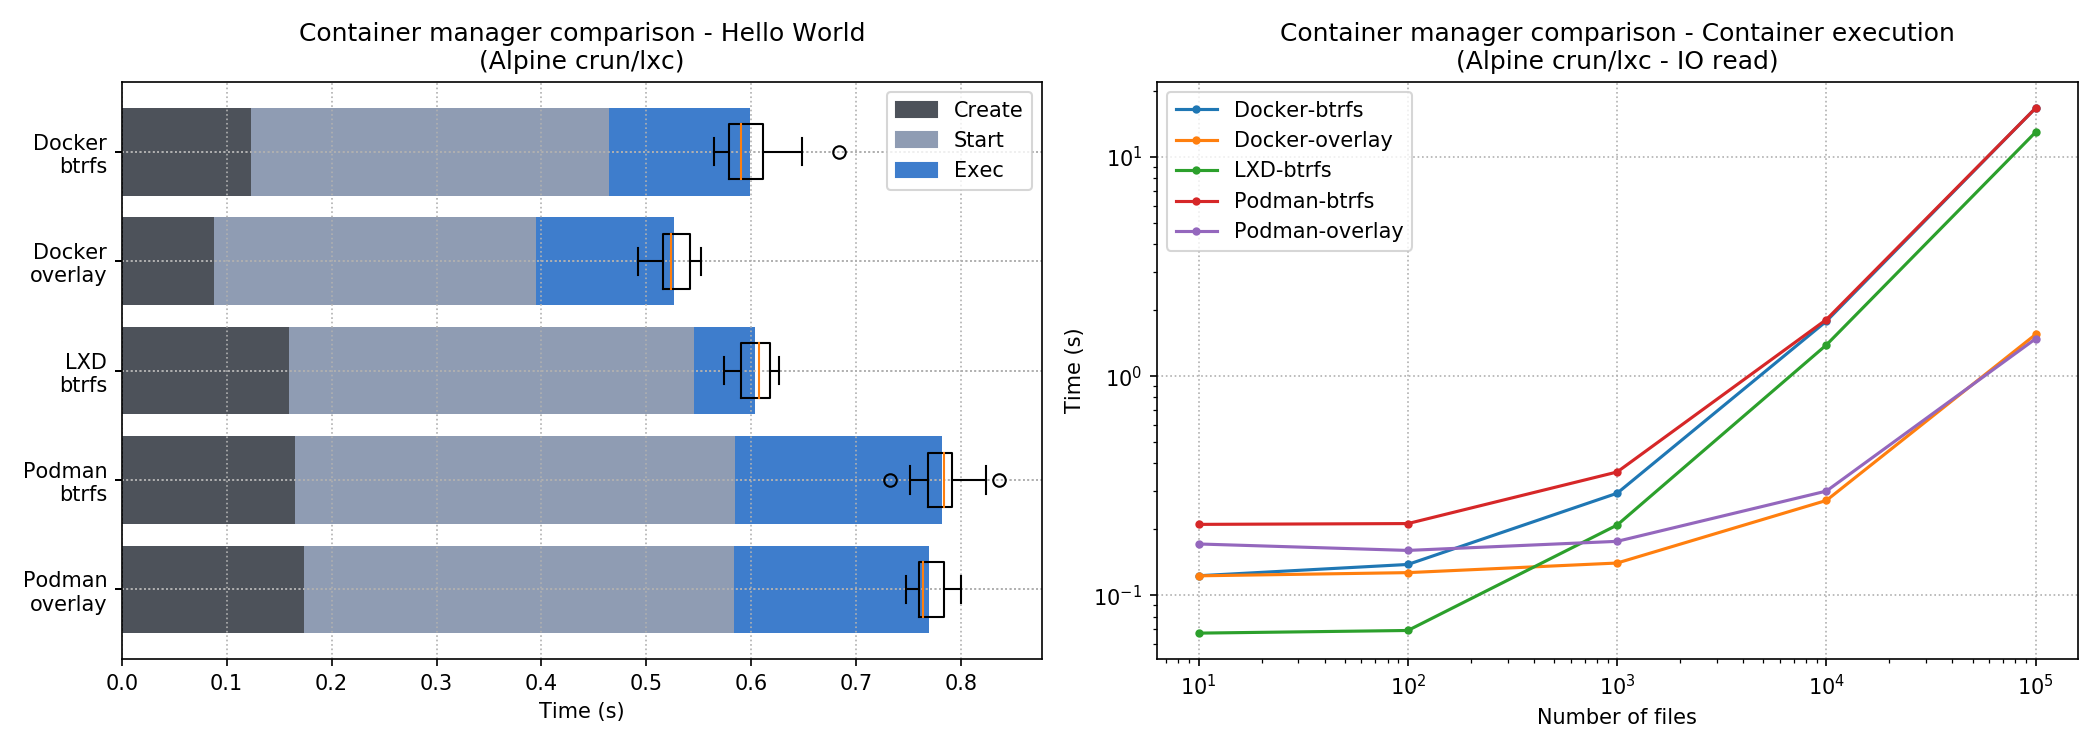
\includegraphics[width=\linewidth]{images/question-1-manager.png}
    \caption{Container manager performance comparison for Alpine containers}
    \label{fig:q1:manager}
  \end{center}
\end{figure}

We can see that Docker is still the best solutions for us, even though none of the other solution presents really bad performances.  Given the relatively young age of Podman, its focus might not be yet fully on performances, but rather on functionnalities.  We can then hope for improvements on this side as time goes, it would be worth check on them later this year, or the next one.  Some interesting things to note regarding Podman's rootless solution:
\begin{itemize}
  \item There is a cost to create rootless containers with Podman compared to going rootfull with the same container manager.  This is very likely caused by the extra steps required to be taken to launch rootless container with all the functionnalities of a rootfull one.  Podman needs first to unshare user and mount namespaces, to be able to make bind mounts on the container filesystem.  It also requires to add a cgroup scope to all the commands that setup the containers, to be sure that the container runtime will later be able to move process created to the cgroup attached to the container.
  \item Because of the lack of \textit{real} root permissions on the machine, rootless containers can not use OverlayFS, instead they use a fuse implementation of the latest, which, as we can see on the right-most graph, induces great performances cost.  It get even worse when doing write operations.
\end{itemize}

\subsubsection{Final configuration}

Based on the previous observations, the ideal configuration would then be:

\begin{center}
\begin{tabular}{rl}
  \textbf{Container manager} & Docker \\
  \textbf{Base image} & Alpine/Centos \\
  \textbf{Storage driver} & overlay2 \\
  \textbf{Container runtime} & crun \\
  \textbf{Control group version} & v1 \\
  \textbf{Rootless containers} & no \\
\end{tabular}
\end{center}

As we can see, the final configuration is not that much different from the original one.  The quick answer to the original questions would be:
\paragraph{}\textit{Compared to other available solutions, how good is the current configuration chosen by INGInious to face the responsiveness challenge of the platform?}  The current configuration is good.  It could be improved, but is definitely not the worse one.  The choice of going with Docker was the most soundfull when INGInious was created, and it is still the case now.  The current storage driver offers great performances for almost every cases, only some specific case, sollicitating a lot of IO operations on big files, can give an advantage to another storage driver, btrfs.  The choice of a Centos base image is not bad either, but the size of the image being greater than Alpine's one, except for the situations where Centos offered better write performances, using Alpine seems to be better.  The move here might then be to go for an hybrid solution, using Centos only in situations where its small writing performance advantage become meaningfull.  
\paragraph{}\textit{How much better could it be?}  As we have seen, changing the current container runtime makes a significant difference.  The c implementation of \texttt{crun} is claimed to be twice as fast as the go implementation of \texttt{runc} by \texttt{crun}'s contributors.  And we can definitely see the difference.  The change of base Image though doesn't show as obvious improvement.
\paragraph{}\textit{How easy would it be to improve it?}  This is the real good news, it truely is super easy to apply the most significant change.  You only need to install \texttt{crun}, reconfigure Docker to use it by default, and you are good to go, no change as to be done to INGInious!  For the base of the base image the story is different though, as it would require to change all the containers images, which is a lot of work.

\section{INGInious ideal solution}
We will here consider the second question:
\begin{center}
  \say{\textit{Could there be a solution tailor-made for the specific case of INGInious?  What would it be?  What would it take to use it?}}
\end{center}

\begin{figure}[h!]
  \begin{center}
    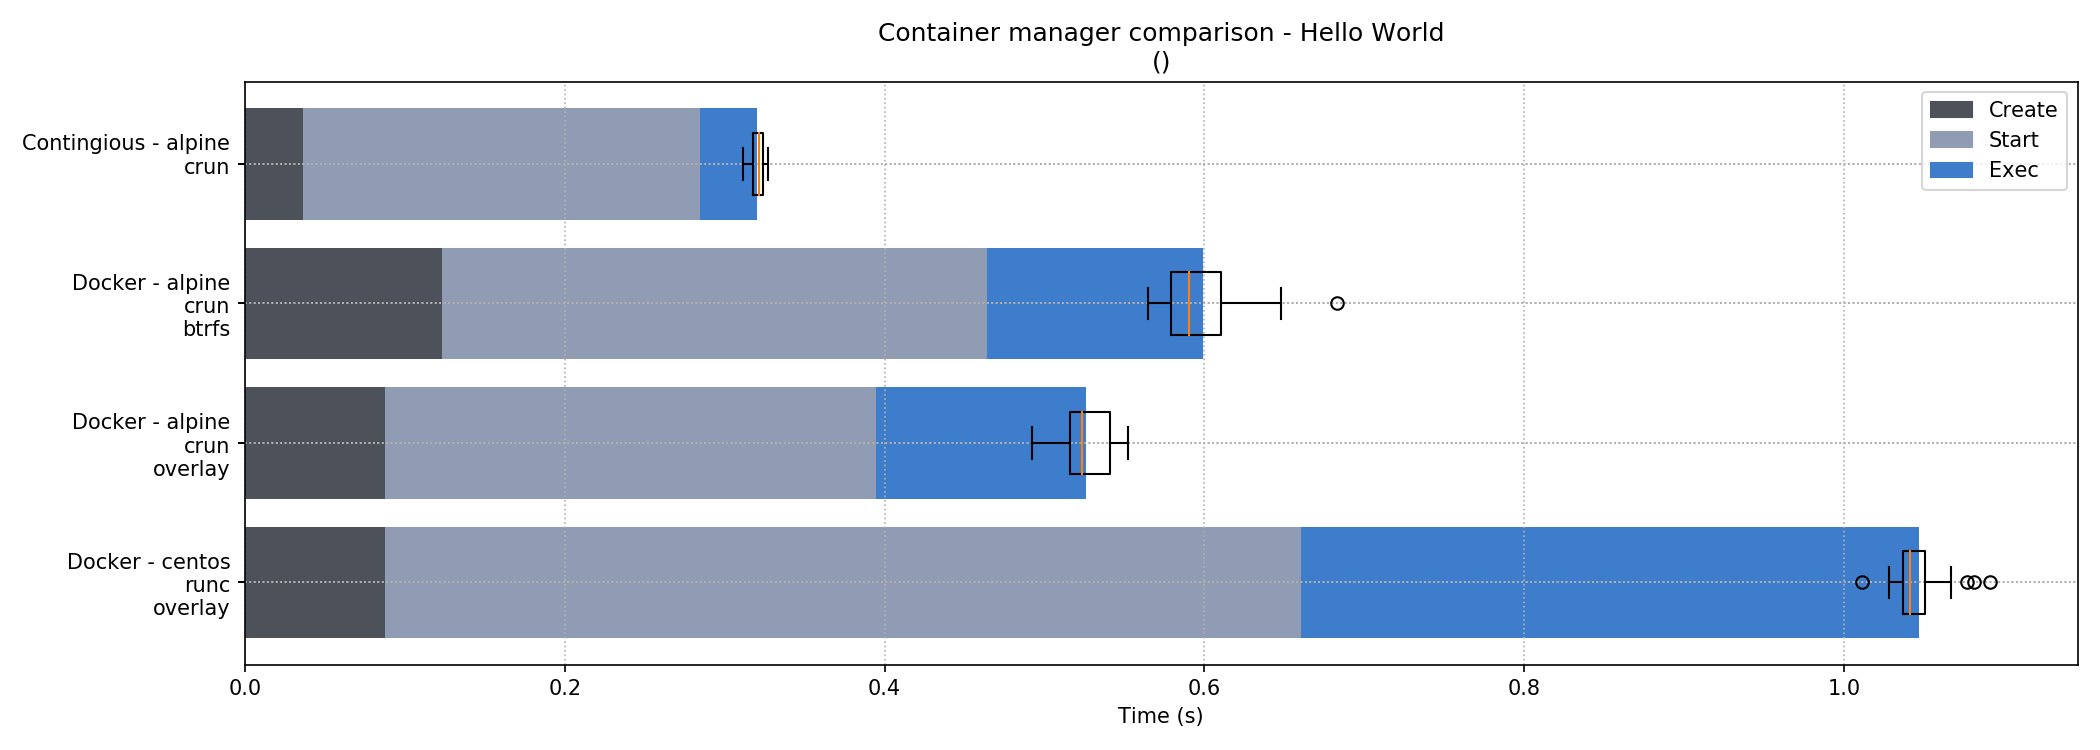
\includegraphics[width=\linewidth]{images/question-2-hello-world.png}
    \caption{Ideal INGInious container manager solution compared to existing ones, Hello World test}
    \label{fig:q2:hello-world}
  \end{center}
\end{figure}

\begin{figure}[h!]
  \begin{center}
    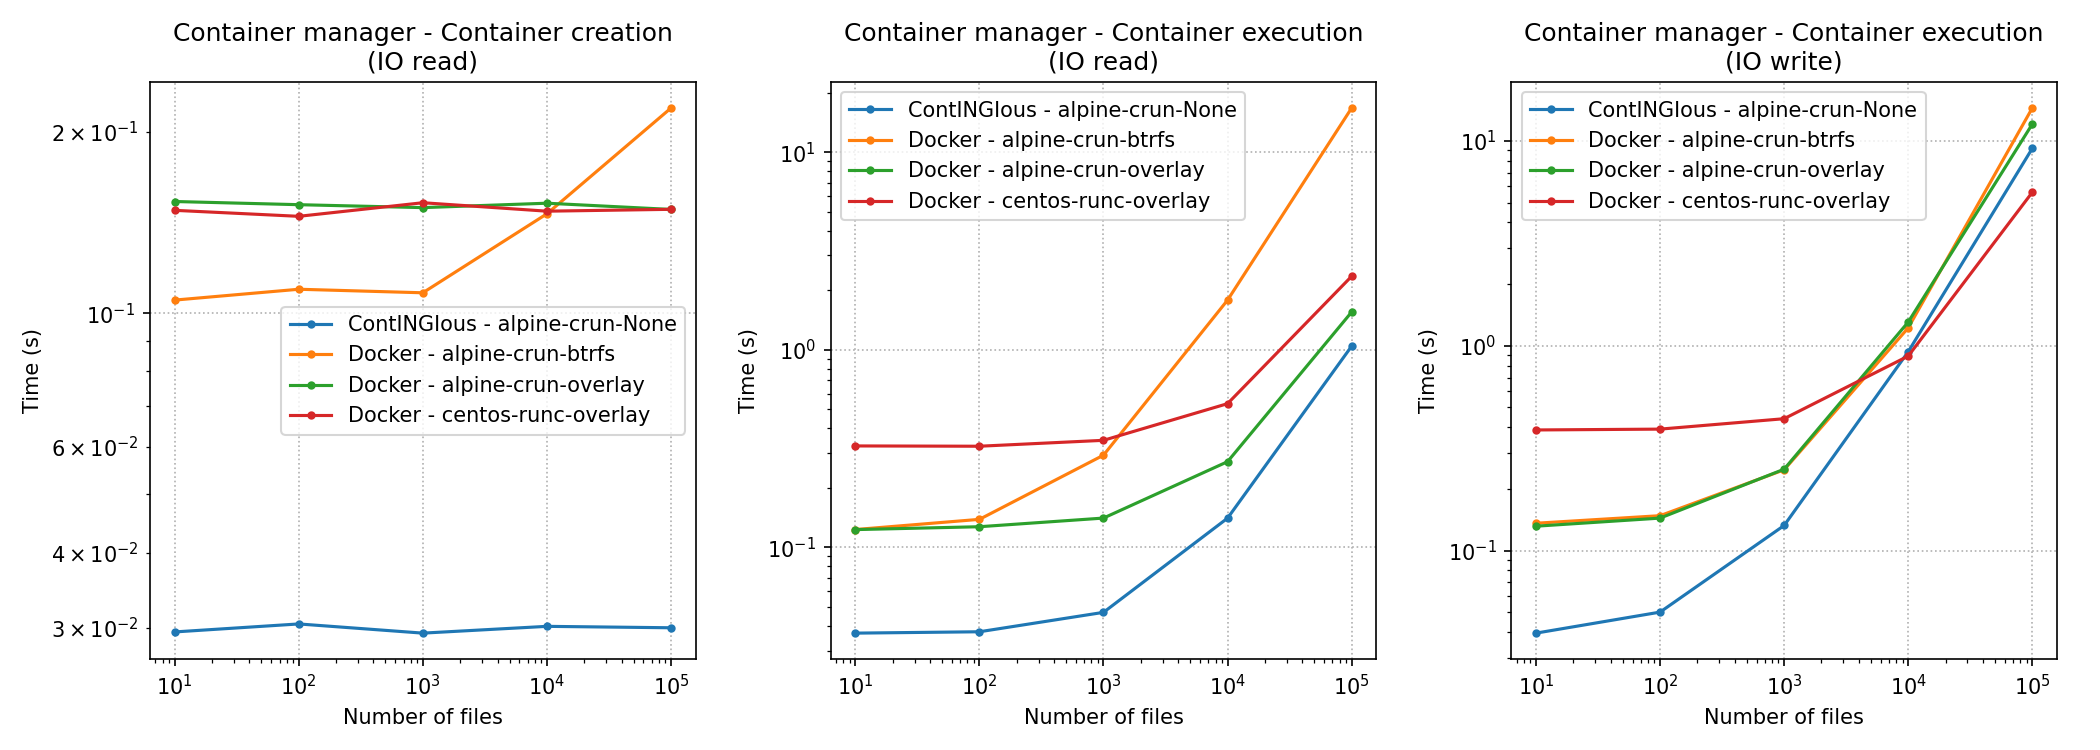
\includegraphics[width=\linewidth]{images/question-2-io.png}
    \caption{Ideal INGInious container manager solution compared to existing ones, IO tests}
    \label{fig:q2:io}
  \end{center}
\end{figure}

\begin{figure}[h!]
  \begin{center}
    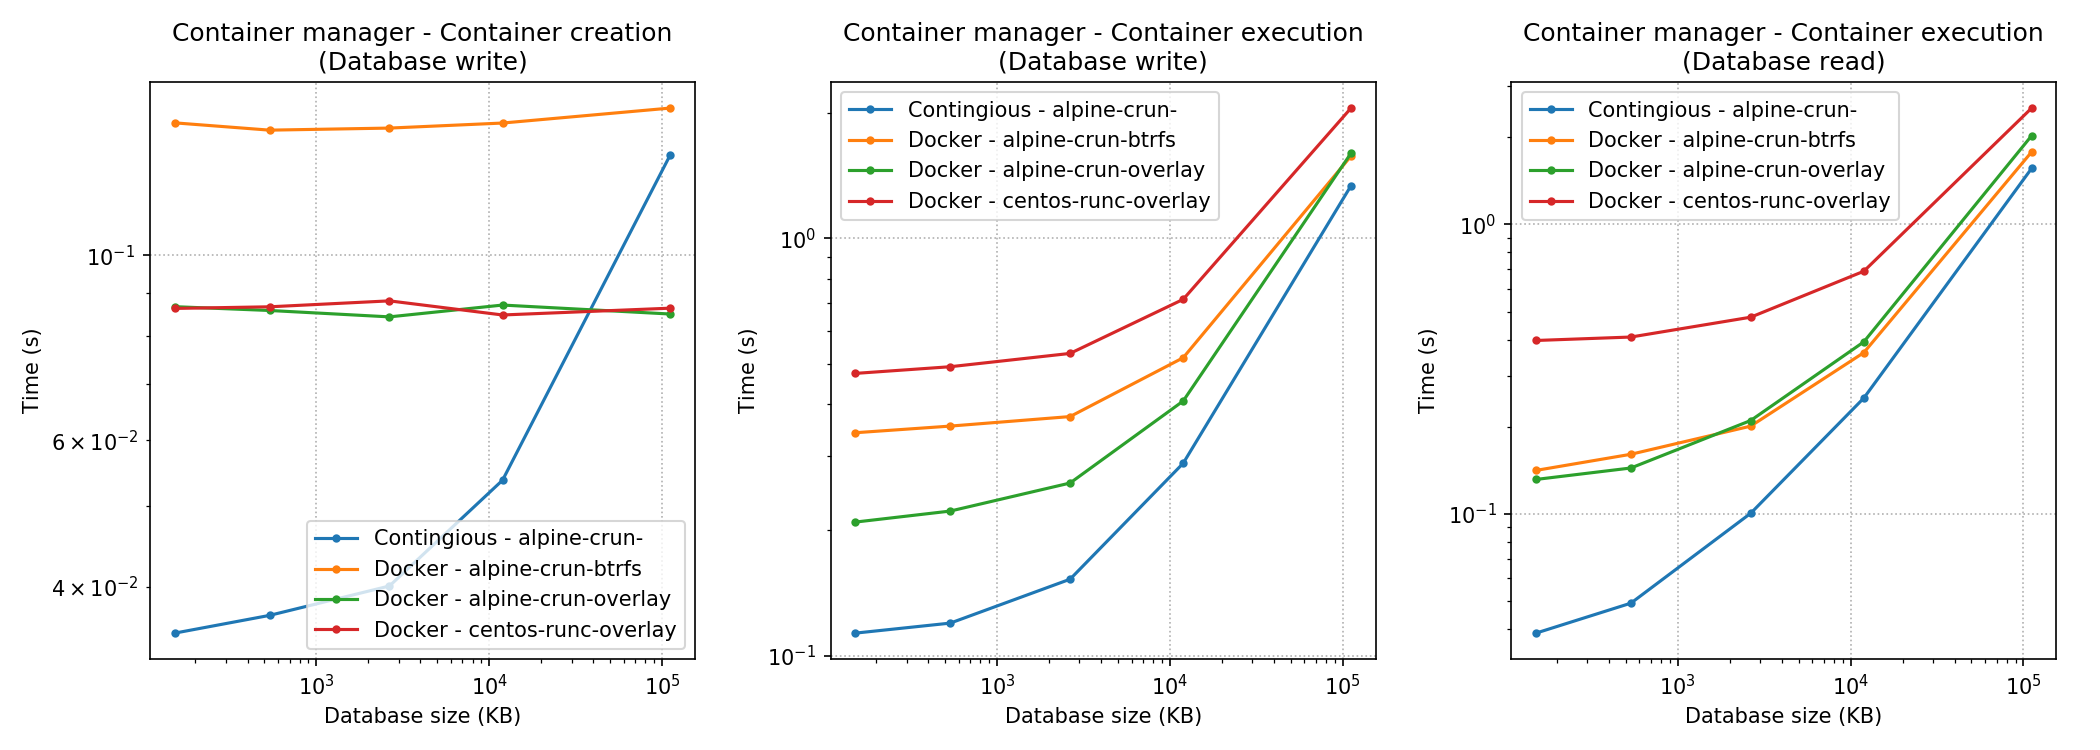
\includegraphics[width=\linewidth]{images/question-2-db.png}
    \caption{Ideal INGInious container manager solution compared to existing ones, Database tests}
    \label{fig:q2:db}
  \end{center}
\end{figure}

\section{INGInious opportunities}
We will here consider the last question:
\begin{center}
  \say{\textit{What would be the cost of providing a stronger/safer isolation to the containers used by INGInious?  What opportunities could it bring?}}
\end{center}

